\documentclass[conference]{IEEEtran}
\usepackage[utf8]{inputenc}
\usepackage[T1]{fontenc}
\usepackage[brazil]{babel}
\usepackage{graphicx}
\usepackage{booktabs}
\usepackage{amsmath}
\usepackage{cite}

\begin{document}

\title{Aprendizado por Reforço com Q-Learning Tabular\\para o Jogo Flappy Bird}

\author{\IEEEauthorblockN{Nome Aluno 1, Nome Aluno 2, Nome Aluno 3}
\IEEEauthorblockA{Disciplina de Inteligência Artificial I -- 2026\\
Instituição\\
emails}}

\maketitle

\begin{abstract}
Este trabalho apresenta um agente baseado em Q-Learning tabular que aprende a jogar Flappy Bird sem conhecimento prévio das regras do jogo. O ambiente foi implementado em Python com a física do jogo original, e o estado foi discretizado em três variáveis (distância horizontal ao próximo cano, diferença vertical ao centro da abertura e velocidade vertical). O agente foi treinado por 40.000 episódios e a política resultante foi avaliada em 100 sementes inéditas, atingindo média de 71,7 canos (mediana 100, limite de 100) e taxa de sucesso de 55\%.
\end{abstract}

\begin{IEEEkeywords}
aprendizado por reforço, Q-Learning, Flappy Bird, jogos.
\end{IEEEkeywords}

\section{Introdução}
Jogos eletrônicos são ambientes clássicos para testar algoritmos de aprendizado por reforço (RL), pois oferecem regras claras, recompensas mensuráveis e simulação barata. O Flappy Bird é um problema simples de enunciar, mas exige temporização precisa de uma única ação (pular) sob dinâmica com gravidade.

\textbf{Objetivo geral:} desenvolver um agente que aprenda a jogar Flappy Bird por tentativa e erro. \textbf{Objetivos específicos:} (i) modelar o jogo como um processo de decisão de Markov discreto; (ii) implementar Q-Learning tabular; (iii) avaliar a política em sementes não vistas no treino.

O restante do artigo está organizado assim: a Seção~II revisa trabalhos relacionados; a Seção~III descreve a metodologia; a Seção~IV apresenta os resultados; a Seção~V conclui.

\section{Trabalhos Relacionados}
% TODO (obrigatorio: >= 4 artigos). Abaixo, base teorica ja verificavel.
% Procure e acrescente 1-2 trabalhos especificos sobre Flappy Bird / jogos simples com RL
% (Google Scholar / IEEE Xplore) e confira os dados bibliograficos antes de entregar.
O Q-Learning foi proposto por Watkins e Dayan~\cite{watkins1992} como método livre de modelo que converge para a função de valor ótima sob condições de visitação suficiente. A formulação geral de RL, incluindo métodos tabulares, é apresentada por Sutton e Barto~\cite{sutton2018}. Mnih et al.~\cite{mnih2015} substituíram a tabela por uma rede neural profunda (DQN) e alcançaram desempenho humano em jogos de Atari, ao custo de maior complexidade e instabilidade de treino; Arulkumaran et al.~\cite{arulkumaran2017} revisam essa linha de métodos profundos. Uma alternativa à abordagem por reforço é a neuroevolução, como o NEAT~\cite{stanley2002}, que evolui topologia e pesos de redes neurais por algoritmo genético.

\emph{Posicionamento:} este trabalho usa Q-Learning tabular, que dispensa redes neurais, é totalmente interpretável (a tabela Q pode ser inspecionada) e permite reproduzir o experimento do zero com poucas linhas de código. % TODO: acrescentar o diferencial do grupo.

\section{Metodologia}
\subsection{Descrição do problema}
O pássaro está em posição horizontal fixa ($x=100$) e deve atravessar aberturas em pares de canos que se movem para a esquerda. A cada quadro, o agente escolhe entre pular ou não fazer nada. O episódio termina quando o pássaro colide com um cano, o chão ou o teto.

\subsection{Ambiente e ferramentas}
O ambiente foi implementado em Python 3.12 (biblioteca padrão), reproduzindo as constantes do jogo original em pygame: tela $400\times600$, chão em $y=520$, raio do pássaro 15, gravidade 0,5 por quadro, velocidade de pulo $-8$, canos com largura 60, abertura 150 e velocidade 3. A altura do topo da abertura é sorteada uniformemente em $[80, 290]$. Novos canos surgem quando o último está a menos de 200 px da borda direita. Matplotlib foi usado nos gráficos e pygame apenas na demonstração visual. Todo o código e os dados estão em \texttt{flappy\_q.py}.

\subsection{Tríade estado--ação--recompensa}
\textbf{Ações:} $a\in\{0,1\}$ (0 = não pular, 1 = pular).

\textbf{Estado:} tripla discretizada $s=(d_x, d_y, v)$, onde $d_x=\lfloor (x_{cano}-x_{p})/20\rfloor$ limitado a $[-3,15]$; $d_y=\lfloor (y_{centro}-y_p)/10\rfloor$ limitado a $[-20,20]$, com $y_{centro}$ o centro da abertura do próximo cano; e $v$ a velocidade vertical inteira limitada a $[-8,6]$. Considera-se próximo cano o primeiro cujo lado direito ainda não passou do pássaro.

\textbf{Recompensa:} $+0{,}1$ por quadro vivo, $+10$ ao ultrapassar um cano e $-100$ ao colidir.

\subsection{Algoritmo}
A atualização de Q-Learning é
\begin{equation}
Q(s,a)\leftarrow Q(s,a)+\alpha\left[r+\gamma\max_{a'}Q(s',a')-Q(s,a)\right],
\end{equation}
com $Q$ nulo na inicialização e $\max_{a'}Q(s',a')=0$ em estados terminais. A política de treino é $\varepsilon$-gulosa: com probabilidade $\varepsilon$ o agente explora, escolhendo pular com probabilidade 0,15 (pular é uma ação rara no jogo, e exploração uniforme gera episódios curtos demais), e com probabilidade $1-\varepsilon$ escolhe a ação de maior $Q$ (empates resolvidos em favor de não pular).

\subsection{Hiperparâmetros}
\begin{table}[h]
\centering
\caption{Hiperparâmetros do treinamento.}
\begin{tabular}{ll}
\toprule
Parâmetro & Valor \\
\midrule
Episódios & 40.000 \\
$\alpha$ & decai linearmente de 0,1 a 0,02 \\
$\gamma$ & 0,99 \\
$\varepsilon$ & decai linearmente de 0,1 a 0,002 até o episódio 20.000 \\
Corte do episódio & 200 canos \\
Semente de treino & 42 \\
\bottomrule
\end{tabular}
\end{table}

\subsection{Validação}
A cada 1.000 episódios a política gulosa é testada em 30 sementes de validação (5000--5029) e a tabela com a melhor média é mantida. A avaliação final usa 100 sementes distintas (10000--10099), com política gulosa e limite de 100 canos por partida. As métricas são média, mediana, mínimo, máximo de canos e taxa de sucesso (partidas que atingem 100 canos).

\section{Resultados}
\begin{figure}[h]
\centering
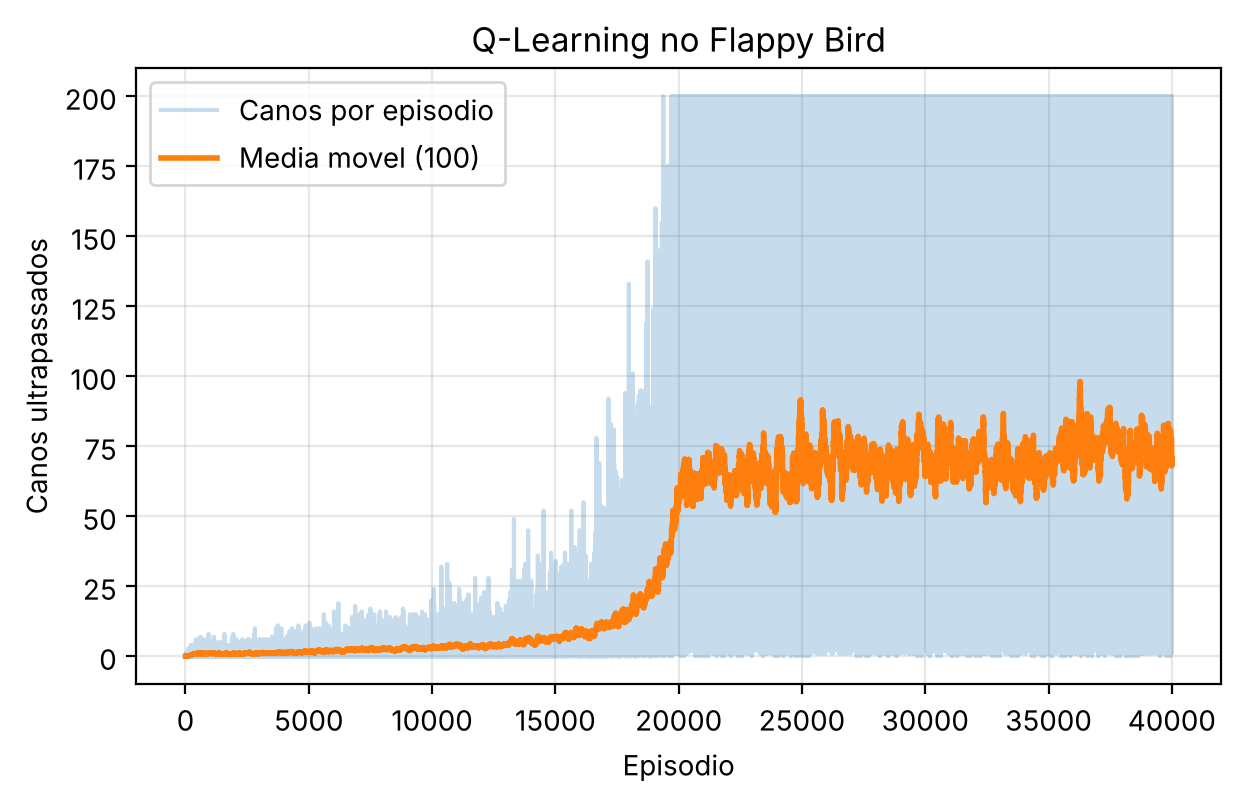
\includegraphics[width=\columnwidth]{grafico_treino.png}
\caption{Canos ultrapassados por episódio de treino (média móvel de 100).}
\end{figure}

\begin{table}[h]
\centering
\caption{Avaliação final (100 sementes inéditas, limite de 100 canos).}
\begin{tabular}{lc}
\toprule
Métrica & Valor \\
\midrule
Média de canos & 71,7 \\
Mediana & 100 \\
Mínimo / Máximo & 1 / 100 \\
Taxa de sucesso & 55\% \\
Estados visitados na tabela Q & 9.039 \\
\bottomrule
\end{tabular}
\end{table}

O aprendizado apresenta duas fases: até cerca de 15.000 episódios o desempenho médio fica abaixo de 10 canos; entre 15.000 e 20.000 há um salto, quando o $\varepsilon$ se aproxima de zero e a política passa a ser explorada. O treino com $\varepsilon$ ainda ativo e $\alpha$ constante mostrou instabilidade (o desempenho chegou a cair em episódios tardios), o que motivou a validação periódica e a seleção do melhor ponto de verificação.

\section{Conclusão}
O Q-Learning tabular aprendeu a jogar Flappy Bird sem conhecimento prévio, chegando a 100 canos em 55\% das partidas inéditas. Como limitações, a discretização grosseira pode agrupar situações distintas e o desempenho varia com a semente. Trabalhos futuros incluem testar outras discretizações, comparar com DQN e repetir o treino com várias sementes para reportar média e desvio padrão. % TODO: incluir essas repeticoes se houver tempo.

\begin{thebibliography}{00}
\bibitem{watkins1992} C. J. C. H. Watkins and P. Dayan, ``Q-learning,'' \emph{Machine Learning}, vol. 8, pp. 279--292, 1992.
\bibitem{sutton2018} R. S. Sutton and A. G. Barto, \emph{Reinforcement Learning: An Introduction}, 2nd ed. MIT Press, 2018.
\bibitem{mnih2015} V. Mnih et al., ``Human-level control through deep reinforcement learning,'' \emph{Nature}, vol. 518, pp. 529--533, 2015.
\bibitem{arulkumaran2017} K. Arulkumaran, M. P. Deisenroth, M. Brundage, and A. A. Bharath, ``Deep reinforcement learning: A brief survey,'' \emph{IEEE Signal Processing Magazine}, vol. 34, no. 6, pp. 26--38, 2017.
\bibitem{stanley2002} K. O. Stanley and R. Miikkulainen, ``Evolving neural networks through augmenting topologies,'' \emph{Evolutionary Computation}, vol. 10, no. 2, pp. 99--127, 2002.
\end{thebibliography}

\end{document}
